\section{Real data analysis}

\begin{frame}{Real networks studied in the paper}
    Real networks studied (directed, unweighted):
    \begin{itemize}
        \item \alert{Digg.com}: social bookmarking site
        \begin{itemize}
            \item Nodes: Digg users
            \item Edges: $a_{ij}=1 \Leftrightarrow$ ``$i$ is a follower of $j$''.
            \item $N = \num{190553}$; $L = \num{1552905}$
        \end{itemize}

        \item \alert{American Physical Society} (APS) articles and citation network
        \begin{itemize}
            \item Nodes: papers (from 1893 to 2009)
            \item Edges: $a_{ij}=1 \Leftrightarrow$ ``$i$ cites $j$''
            \item $N = \num{450056}$; $L = \num{4690967}$
        \end{itemize}
    \end{itemize}
    \vspace{1em}
    Estimator of node fitness: \alert{total relevance} of node $i$
    \[
        T_i = \sum_t r_i(t)
    \]
\end{frame}

\begin{frame}{PageRank performance on real data}
    \begin{figure}
        \begin{columns}
            \column{0.55\textwidth}
                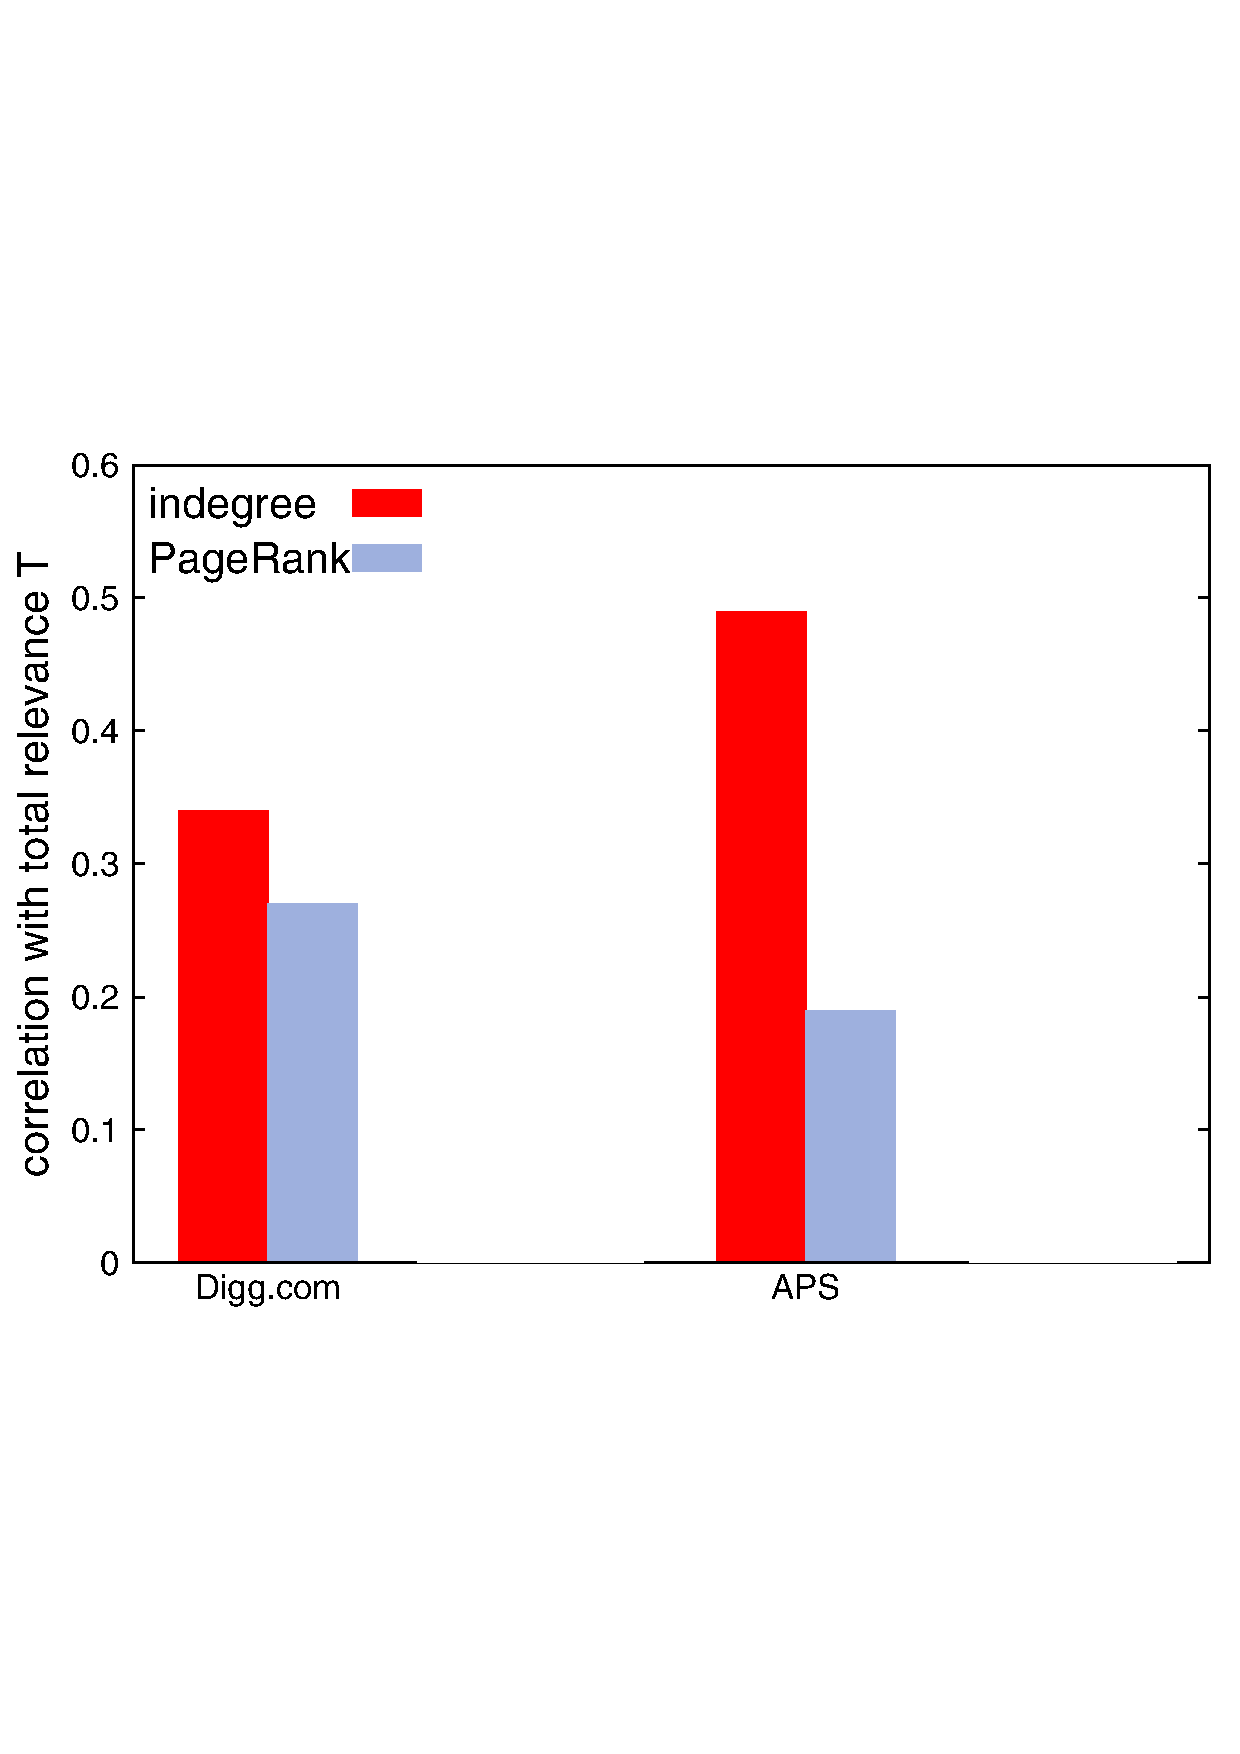
\includegraphics[width=1.1\textwidth]{figures/PageRank_realdata}
            \column{0.45\textwidth}
                \begin{footnotesize}
                    \begin{itemize}
                        \item \alert{Digg.com}: activity and relevance decay s.t. PageRank is maximally correlated with indegree in RM simulations with power-law decay.
                        \item \alert{APS}: \\ activity decays immediately, \\ relevance decays progressively.
                    \end{itemize}
                \end{footnotesize}
        \end{columns}
        \caption{Comparison of PageRank and indegree correlation with total relevance $T_i$ in real data. APS: PageRank strongly biased towards old nodes, because papers can only be cited by more recent papers.}
    \end{figure}
\end{frame}
